   \title{
Dynamic Abstract Neural Computing\\with\ Electronic Simulation\\(DANCES)  Version \emph{\MyVersion}\\
\iflatexml
\else
\vskip 1 cm
\small{The true physics, physiology, computing, and information science\\behind neuronal operation}
\fi
}

\author{János Végh}
\date{\today}
\lxKeywords{dynamic neural modelling, Hodgkin-Huxley model, unified neuron model, neural information, neural computing, physics for biology, time-aware computing}
%============================================================
\begin{lxNavbar}
%
\includegraphics[width=0.42\textwidth]{../graphics/BrainElectronics.png}

\includegraphics[width=0.375\textwidth]{../graphics/neurer.png}
Dynamic Abstract Neural Computing\\ with Electronic Simulation\\
\small{The true physics, physiology, computing,and information science\\behind neuronal operation}\\
(DANCES) Version \emph{\MyVersion}\\
@\today
\lxContextTOC
%\\
\href{../../simulator/ToIssue.html}{Report issue}
\href{../manual.pdf}{Manual in .PDF form}
\href{../../simulator/index.html}{Simulator}
\href{../../simulator/ToCode.html}{Code}
\href{../../doxy/HTML/index.html}{Code documentation}
\href{https://github.com/jvegh/Dynamic-Abstract-Neural-Computing/graphs/code-frequency}{Development pace}
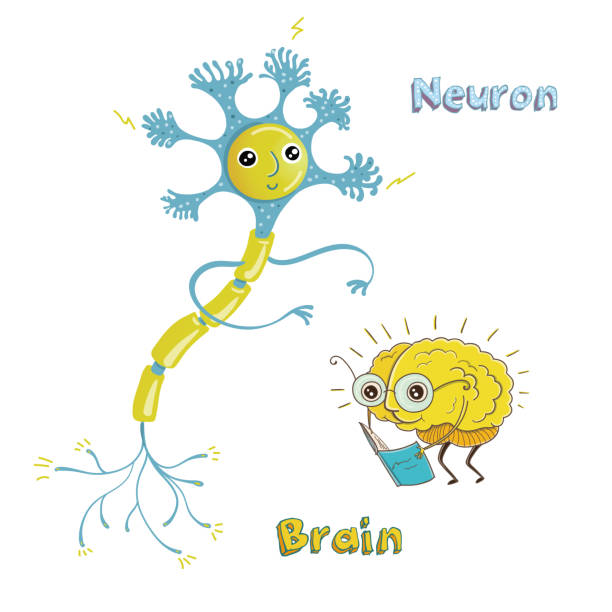
\includegraphics[width=0.41\textwidth]{../graphics/NeuronAndBrain.jpg}
\end{lxNavbar}

